\chapter{Evaluation Metrics}
\label{ch:eval-metrics}

Model-based metrics for evaluating machine translation such as BLEURT \cite{sellam-etal-2020-bleurt}, ESIM \cite{mathur-etal-2019-ESIM}, and YiSi \cite{lo-2019-yisi} have recently attracted attention due to their superior correlation with human judgments \cite{WMT19-metrics-proceedings}. However, \bleu~\cite{papineni-etal-2002-bleu} remains  the most widely used corpus-level MT metric. It correlates reasonably well with human judgments, and moreover is easy to understand and cheap to calculate, requiring only reference translations in the target language. By contrast, model-based metrics require tuning on thousands of examples of human evaluation for every new target language or domain \cite{sellam-etal-2020-bleurt}. Model-based metric scores are also opaque and can hide undesirable biases, as can be seen in Table~\ref{tab:bleurt-bias}.


\begin{table}[ht]
    \centering
    %\footnotesize
    \begin{tabular}{l l l }
Reference:& \multicolumn{2}{l}{You must be a doctor.} \\
Hypothesis: & \multicolumn{2}{l}{$\rule{1cm}{0.15mm}$ must be a doctor.} \\
    % & You &	~0.990 \\
    & He	&-0.735 \\
    %& Alexandra & -0.888 \\
    %& Alexander & -0.975 \\
    & Joe & -0.975 \\
    & Sue & -1.043 \\
    & She	 &-1.100 \\\hline
Reference:& \multicolumn{2}{l}{It is the greatest country in the world.} \\
Hypothesis:& \multicolumn{2}{l}{$\rule{1cm}{0.15mm}$ is the greatest country in the world.} \\
    % & It	& ~0.957 \\
    & France &	-0.022 \\
    & America	& -0.060 \\
    & Russia &	-0.161 \\
    %& China  & -0.166 \\
    %& USA    & -0.168 \\
    %& India   &	-0.211 \\
    & Canada  & -0.309 
    \end{tabular}
    \caption{A demonstration of BLEURT's internal biases; model-free metrics like BLEU would consider each of the errors above to be equally wrong.}
    \label{tab:bleurt-bias}
\end{table}

The source of model-based metrics' (e.g. BLEURT) correlative superiority over model-free metrics (e.g. BLEU) appears to be the former's ability to focus evaluation on \textit{adequacy}, while the latter are overly focused on \textit{fluency}. BLEU and most other generation metrics consider each output \textit{token} equally. Since natural language is dominated by a few high-count types, an MT model that concentrates on getting its \textit{if}s, \textit{and}s and \textit{but}s right will benefit from BLEU in the long run more than one that gets its \textit{xylophone}s, \textit{peripatetic}s, and \textit{defenestrate}s right. Can we derive a metric with the discriminating power of BLEURT that does not share its bias or expense and is as interpretable as BLEU? 

As it turns out, the metric may already exist and be in common use. Information extraction and other areas concerned with classification have long used both \textit{micro averaging}, which treats each token equally, and \textit{macro averaging}, which instead treats each \textit{type} equally, when evaluating. The latter in particular is useful when seeking to avoid results dominated by overly frequent types.  In this work we take a classification-based approach to evaluating machine translation in order to obtain an easy-to-calculate metric that focuses on adequacy as much as BLEURT but does not have the expensive overhead, opacity, or bias of model-based methods. 


Our contributions are as follows:
We consider MT as a classification task, and thus admit \maf1 as a legitimate approach to evaluation~(Section ~\ref{sec:mt-as-cls}). 
We show that \maf1 is competitive with other popular methods at tracking human judgments in translation (Section~\ref{sec:wmt-metrics}). 
We offer an additional justification of \maf1 as a performance indicator on adequacy-focused downstream tasks such as cross-lingual information retrieval (Section \ref{sec:clir}). 
Finally, we demonstrate that \maf1 is just as good as the expensive BLEURT at discriminating between structurally different MT approaches in a way \bleu\ cannot, especially regarding the adequacy of generated text, and provide a novel approach to qualitative analysis of the effect of metrics choice on quantitative evaluation (Section \ref{sec:unmt}).




\section{NMT as Classification}
\label{sec:mt-as-cls}
Neural machine translation (NMT) models are often viewed as pairs of encoder-decoder networks.
Viewing NMT as such is useful in practice for implementation; however, such a view is inadequate for theoretical analysis. 
\citet{gowda-may-2020-finding} provide a high-level view of NMT as two fundamental ML components: an autoregressor and a classifier. 
Specifically, NMT is viewed as a multi-class classifier that operates on representations from an autoregressor.
We may thus consider classifier-based evaluation metrics.


Consider a test corpus, $T = \{ (x^{(i)}, h^{(i)}, y^{(i)}) | i = 1,2,3...m \}$ where $x^{(i)}$, $h^{(i)}$, and $y^{(i)}$ are source, system hypothesis, and reference translation, respectively. Let $x = \{x^{(i)} \forall i\}$ and similar for $h$ and $y$.  Let $V_h, V_y, V_{h\cap y},$ and $V$ be the vocabulary of $h$, the vocabulary of $y$, $V_h \cap V_y$, and $V_h \cup V_y$, respectively.
For each class $c \in V$, 
\begin{align*}
 \textsc{Preds}(c) &= \sum_{i=1}^m C(c, h^{(i)})\\
 \textsc{Refs}(c) &= \sum_{i=1}^m C(c, y^{(i)})\\
\textsc{Match}(c) &= \sum_{i=1}^m min\{C(c, h^{(i)}), C(c, y^{(i)})\} 
\end{align*}
\noindent where $C(c, a)$  counts the number of tokens of type $c$ in sequence $a$~\cite{papineni-etal-2002-bleu}. 
For each class $c \in V_{h \cap y}$, precision ($P_c$), recall ($R_c$), and $F_\beta$ measure ($F_{\beta;c}$) are computed as follows:\footnote{We consider $F_{\beta;c}$ for $c \not\in V_{h \cap y}$ to be 0.}
\begin{align*}
    P_c &= \frac{\textsc{Match}(c)}{\textsc{Preds}(c)} ; \hspace{5mm} R_c = \frac{\textsc{Match}(c)}{\textsc{Refs}(c)} \\
    F_{\beta;c} &= (1 + \beta^2)  \frac{ P_c \times R_c}{ \beta^2 \times P_c + R_c}
\end{align*}

The \textit{macro-average} consolidates individual performance by averaging by type, while the \textit{micro-average} averages by token:  
\begin{align*}
\maf\beta &= \frac{\sum_{c \in V} F_{\beta;c}} {|V|}\\
\mif\beta &= \frac{\sum_{c\in V} f(c) \times F_{\beta;c}} {\sum_{c'\in V} f(c')}
\end{align*}
\noindent where $f(c) = \textsc{Refs}(c)+k$ for smoothing factor $k$.\footnote{We use $k=1$. When $k \rightarrow \infty, \space \mif\beta \rightarrow \maf\beta. $} We scale $\maf\beta$ and $\mif\beta$ values to percentile, similar to \bleu, for the sake of easier readability. 


\section{Justification for \texorpdfstring{\maf1}{MacroF1}}
\label{sec:justific}

In the following sections, we verify and justify the utility of \maf1 while also offering a comparison with popular alternatives such as \mif1, \bleu, \chrf{1}, and BLEURT.\footnote{\bleu\ and \chrf1 scores reported in this work are computed with \textsc{SacreBleu}; see the Appendix for details.
BLEURT scores are from the \textit{base} model \citep{sellam-etal-2020-bleurt}. We consider two varieties of averaging to obtain a corpus-level metric from the segment-level BLEURT: mean and median of segment-level scores per corpus.
}
We use Kendall's rank correlation coefficient, $\tau$, to compute the association between metrics and human judgments.
Correlations with p-values smaller than $\alpha=0.05$ are considered to be statistically significant.


\begin{figure}
    \centering
    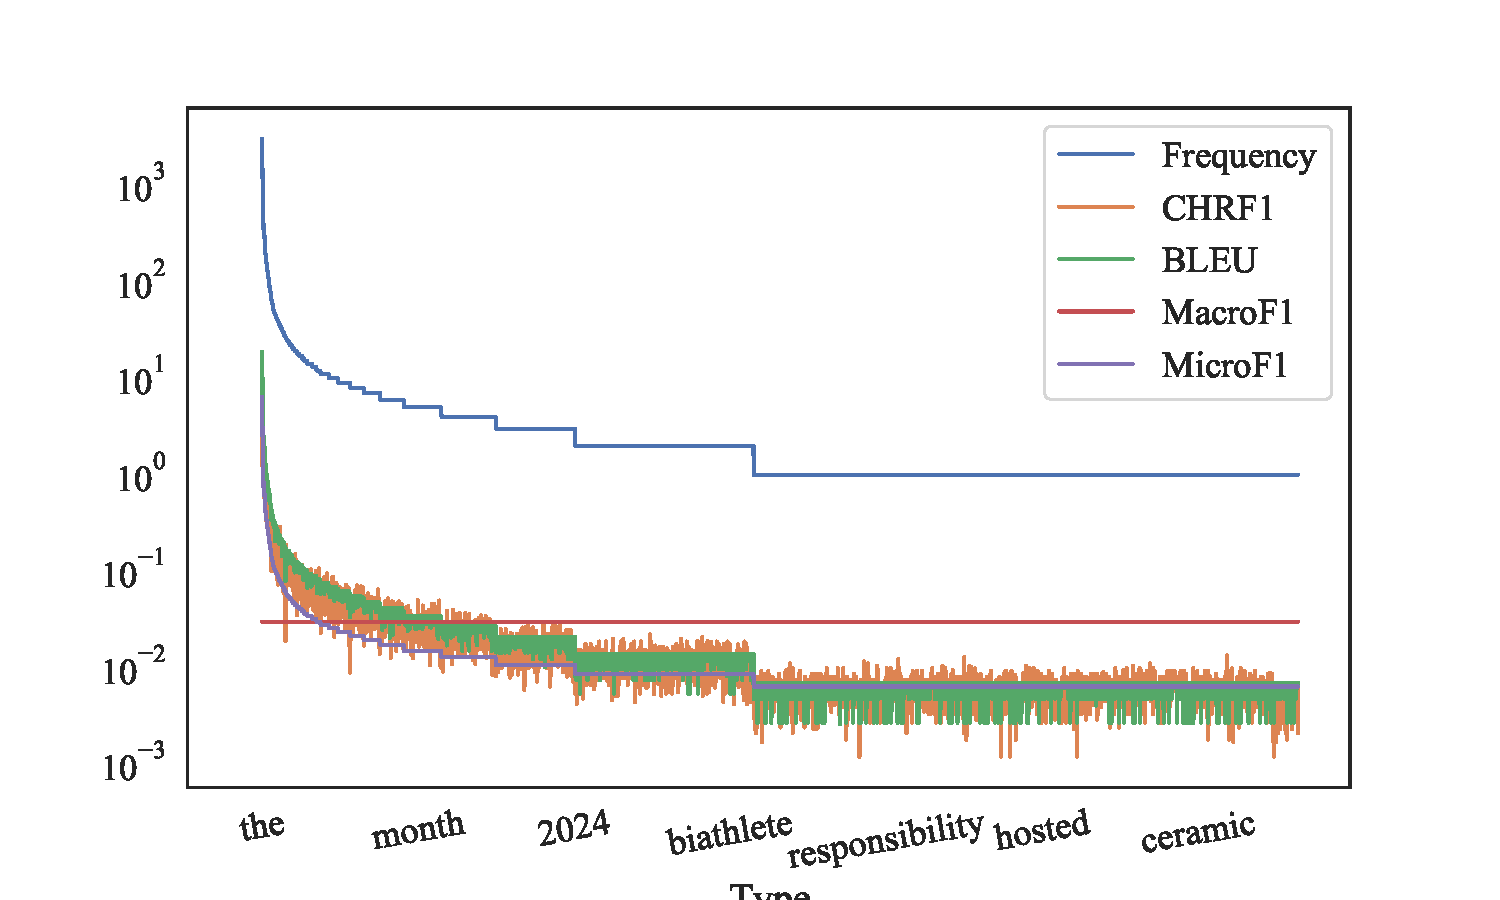
\includegraphics[width=\textwidth]{img/macroavg/bleu-chrf-macro-micro-swapin-lenmatch.pdf}
    \caption{Caption}
    \label{fig:bleu-damage}
\end{figure}

\subsection{Data-to-Text: WebNLG}
\label{sec:webnlg}


\begin{table}[ht]
%    \footnotesize
    \centering
    \begin{tabular}{lrr}
Name & Fluency \& Grammar & Semantics \\ \hline\hline
\bleu\  & \insig.444 & \insig.500 \\
\chrf1 & \insig.278    & .778   \\
\maf1  & \insig.222    & .722   \\
\mif1  & \insig.333    & .611   \\ \hline
\blrtmn & \insig.444   & .833   \\
\blrtmd & .611  & .667   \\
\end{tabular}
    \caption{\small WebNLG data-to-text task: Kendall's $\tau$ between system-level MT metric scores and human judgments.
    Fluency and grammar are correlated identically by all metrics.
    Values that are \textit{not} significant at $\alpha=0.05$ are indicated by \insig{}.}
    \label{tab:webnlg-kendall}
\end{table}


We use the 2017 WebNLG Challenge dataset \cite{gardent2017webNLG-corpus, shimorina2018webnlg-human-eval}\footnote{\url{https://gitlab.com/webnlg/webnlg-human-evaluation}} to analyze the differences between micro- and macro- averaging. 
WebNLG is a task of generating English text for sets of triples extracted from DBPedia.
Human annotations are available for a sample of 223 records each from nine NLG systems.
The human judgments provided have three linguistic aspects---fluency, grammar, and semantics\footnote{Fluency and grammar, which are elicited with nearly identical directions \cite{gardent2017webNLG-corpus}, are identically correlated.}---which enable us to perform a fine grained analysis of our metrics.
We compute Kendall's $\tau$ between metrics and human judgments, which are reported in Table~\ref{tab:webnlg-kendall}.

As seen in Table~\ref{tab:webnlg-kendall}, the metrics exhibit much variance in agreements with human judgments. %Fluency and grammar display same correlations and hence are com  
For instance, \blrtmd\ is the best indicator of fluency and grammar, however \blrtmn\ is best on semantics. 
BLEURT, being a \textit{model-based} measure that is directly trained on human judgments, scores relatively higher than others.
Considering the model-free metrics, \chrf1 does well on semantics but poorly on fluency and grammar compared to \bleu.
Not surprisingly, both \mif1 and \maf1, which rely solely on unigrams, are poor indicators of fluency and grammar compared to \bleu, however \maf1 is clearly a better indicator of semantics than \bleu. 
The discrepancy between \mif1 and \maf1 regarding their agreement with fluency, grammar, and semantics is expected: micro-averaging pays more attention to function words (as they are frequent types) that contribute to fluency and grammar whereas macro-averaging pays relatively more attention to the content words that contribute to semantic adequacy. 

The take away from this analysis is as follows: \maf1 is a strong indicator of semantic adequacy, however, it is a poor indicator of fluency. We recommend using either \maf1 or \chrf1 when semantic adequacy and not fluency is a desired goal.

\subsection{Machine Translation: WMT Metrics}
\label{sec:wmt-metrics}

\begin{table*}[ht!]
    %\footnotesize
    %\small
    \centering
    
\begin{tabular}{r r l r r r r r }
Year & Pairs  & & $\star$\bleu\ & \bleu\ & \maf1 & \mif1 & \chrf1 \\ \hline\hline
\multirow{3}{*}{ 2019 } 
    & \multirow{3}{*}{18}
     & Mean   & .751 & .771 & .821 & .818 & .841  \\ 
   & & Median & .782 & .752 & .844 & .844 & .875  \\
   & & Wins   &     3 &     3 &  \textbf{6}    &     3 &   5 \\ \hline
\multirow{3}{*}{ 2018 } 
  & \multirow{3}{*}{14}
   & Mean   & .858 & .857 & .875 & .873 & .902  \\ 
  & & Median & .868 & .868 & .901 & .879 & .919  \\
  & & Wins    &  1  &  2 & 3 &  2 &  \textbf{6}\\ \hline  
\multirow{3}{*}{ 2017 }
   & \multirow{3}{*}{13}
    & Mean   & .752 & .713 & .714 & .742 & .804 \\  
  & & Median & .758 & .733 & .735 & .728 & .791 \\
  & & Wins   & 5 & 4 & 2 & 2 & \textbf{6} \\
\end{tabular}   
\caption{WMT 2017--19 Metrics task: Mean and median Kendall's $\tau$ between MT metrics and human judgments.
Correlations that are not significant at $\alpha=0.05$ are excluded from the calculation of mean, and median, and wins.
See Appendix Tables \ref{tab:wmt19-kendall}, \ref{tab:wmt18-kendall}, and \ref{tab:wmt17-kendall} for full details.
$\star$\bleu\ is pre-computed scores available in the metrics packages.
In 2018 and 2019, both \maf1 and \mif1 outperform \bleu, \maf1 outperforms \mif1.
\chrf1 has strongest mean and median agreements across the years.
Judging based on the number of wins, \maf1 has steady progress over the years, and outperforms others in 2019.
}
\label{tab:wmt-summary}
\end{table*}

In this section, we verify how well the metrics agree with human judgments using Workshop on Machine Translation (WMT) metrics task datasets for 2017--2019~\cite{WMT17-metrics,WMT18-metrics,WMT19-metrics-proceedings}.\footnote{\url{http://www.statmt.org/wmt19/metrics-task.html}}
We first compute scores from each MT metric, and then calculate the correlation $\tau$ with human judgments.

As there are many language pairs and translation directions in each year, we report only the mean and median of $\tau$, and number of wins per metric for each year in Table \ref{tab:wmt-summary}.
We have excluded BLEURT from comparison in this section since the BLEURT models are fine-tuned on the same datasets on which we are evaluating the other methods.\footnote{\url{https://github.com/google-research/bleurt}}
\chrf1 has the strongest mean and median agreement with human judgments across the years.
In 2018 and 2019, both \maf1 and \mif1 mean and median agreements outperform \bleu\, whereas in 2017 \bleu\ was better than \maf1 and \mif1.


As seen in Section~\ref{sec:webnlg}, \maf1 weighs towards semantics whereas \mif1 and \bleu\ weigh towards fluency and grammar.
This indicates that recent MT systems are mostly fluent, and adequacy is the key discriminating factor amongst them.
\bleu\ served well in the early era of statistical MT when fluency was a harder objective. 
Recent advancements in neural MT models such as Transformers \cite{vaswani2017attention} produce fluent outputs, and have brought us to an era where semantic adequacy is the focus.


% save it for the slides
%We envision that the methods such as \maf1 that emphasize the long tail be more successful in the future years, and this vision is inline with \citet{steedman-2008-last}:
%One day, either because of the demise of Moore’slaw, or simply because we have done all the easy stuff, the Long Tail will come back to haunt us.
%\textit{``One day, ... simply because we have done all the easy stuff, the Long Tail will come back to haunt us.''}

\subsection{Downstream Task: Cross-Lingual Information Retrieval}
\label{sec:clir}
In this section, we determine correlation between MT metrics and  downstream cross-lingual information retrieval (CLIR) tasks.
CLIR is a kind of information retrieval (IR) task in which documents in one language are retrieved given queries in another~\cite{grefenstette2012CLIR}. 
A practical solution to CLIR is to translate source documents into the query language using an MT model, then use a monolingual IR system to match queries with translated documents. 
Correlation between MT and IR metrics is accomplished in the following steps: 
\begin{enumerate}[noitemsep,topsep=0pt]
 \item Build a set of MT models and measure their performance using MT metrics.
 \item Using each MT model in the set, translate all source documents to the target language, build an IR model, and measure IR performance on translated documents.
 \item For each MT metric, find the correlation between the set of MT scores and their corresponding set of IR scores.
 The MT metric that has a stronger correlation with the IR metric(s) is more useful than the ones with weaker correlations.
\item Repeat the above steps on many languages to verify the generalizability of findings.
\end{enumerate}


An essential resource of this analysis is a dataset with human annotations for computing MT and IR performances.
We conduct experiments on two datasets: firstly, on data from the 2020 workshop on \textit{Cross-Language Search and Summarization of Text and Speech} (CLSSTS) \cite{zavorin-etal-2020-corpora}, and secondly, on data originally from Europarl, prepared by \citet{lignos-etal-2019-MT-IR} (Europarl).

\subsubsection{CLSSTS Datasets}
\label{sec:material}

\begin{table*}[ht]
    %\footnotesize
    \begin{tabular}{l l l r r r r r r }
 & Domain & IR Score & \bleu\ & \maf1 & \mif1 & \chrf1 & \blrtmn & \blrtmd \\\hline\hline

\multirow{4}{*}{LT-EN} 
& \multirow{2}{*}{In} 
  & AQWV & .429 & \insig.363 & \textbf{.508} & \insig.385 & .451  & .420 \\
& & MAP  & .495  & .429      & \textbf{.575} & .451       & .473  & .486 \\
& \multirow{2}{*}{In+Ext}
   & AQWV & \insig.345 & \textbf{.527} & .491  & .491 & .491 & .477 \\
&  & MAP  & \insig.273 & \insig\textbf{.455} & \insig.418 & \insig.418 & \insig.418 & \insig.404 \\\hline
\multirow{4}{*}{PS-EN}
  & \multirow{2}{*}{In} 
    & AQWV  & .559 & \textbf{.653} & .574 & .581 & .584 & .581  \\
  & & MAP   & .493 & \textbf{.632} & .487 & .494 & .558 & .554 \\
  & \multirow{2}{*}{In+Ext}
    & AQWV   & .589 & \textbf{.682} & .593 & .583 & .581 & .571 \\
  & & MAP    & .519 & \textbf{.637} & .523 & .482 & .536 & .526 \\\hline
\multirow{4}{*}{BG-EN}
 & \multirow{2}{*}{In} 
    & AQWV   & \insig.455 & \textbf{.550}   & .527  & \insig.382 & \insig.418  & .418 \\ 
 &  & MAP    &  .491      &  \textbf{.661}  & .564  &  .491       & .527       & .527 \\ 
 & \multirow{2}{*}{In+ext}
    & AQWV   & \insig.257 & \textbf{.500}       & \insig.330 & \insig.404 & \insig.367 & \insig.367 \\
 &  & MAP   & \insig.183 & \insig\textbf{.426} & \insig.257 & \insig.330 & \insig.294 & \insig.294 
\end{tabular} 
\caption{CLSSTS CLIR task: Kendall's $\tau$ between IR and MT metrics under study.
The rows with Domain=In are where MT and IR scores are computed on the same set of documents, whereas Domain=In+Ext are where IR scores are computed on a larger set of documents that is a superset of segments on which MT scores are computed.
\textbf{Bold} values are the best correlations achieved in a row-wise setting; values with \insig~ are \textit{not} significant at $\alpha=0.05$.}
\label{tab:material-kendall}
\end{table*}


CLSSTS datasets contain queries in English~(EN), and documents in many source languages along with their human translations, as well as query-document relevance judgments. 
We use three source languages: Lithuanian~(LT), Pashto~(PS), and Bulgarian~(BG).
The performance of this CLIR task is evaluated using two IR measures: Actual Query Weighted Value (AQWV) and Mean Average Precision (MAP).
AQWV\footnote{\href{https://www.nist.gov/system/files/documents/2017/10/26/aqwv\_derivation.pdf}{https://www.nist.gov/system/files/documents-/2017/10/26/aqwv\_derivation.pdf}} is derived from Actual Term Weighted Value (ATWV) metric \cite{wegmann2013ATWV}. 
We use a single CLIR system \cite{boschee-etal-2019-saral} with the same IR settings for all MT models in the set, and measure Kendall's $\tau$ between MT and IR measures.
The results, in Table~\ref{tab:material-kendall}, show that \maf1 is the strongest indicator of CLIR downstream task performance in five out of six settings.
AQWV and MAP have a similar trend in agreement to the MT metrics.
\chrf1 and BLEURT, which are strong contenders when generated text is directly evaluated by humans, do not indicate CLIR task performance as well as \maf1, as CLIR tasks require faithful meaning equivalence across the language boundary, and human translators can mistake fluent output for proper translations \cite{callison-burch-etal-2007-meta}. 


\subsubsection{Europarl Datasets}
\label{sec:lignos-etal}

\begin{table}[ht]
    %\footnotesize
    \centering
\begin{tabular}{l@{\hspace{1mm}} r@{\hspace{1mm}} r@{\hspace{1mm}} r@{\hspace{1mm}} r@{\hspace{1.2mm}} r@{\hspace{1.2mm}} r}
 & \bleu\ & \maf1 & \mif1 & \chrf1 & $\overline{\text{BT}}$ & $\widetilde{\text{BT}}$ \\ \hline\hline
\multirow{1}{*}{ CS-EN } 
 & .850 & .867 & .850 & .850 & \textbf{.900} & .867 \\ 
\multirow{1}{*}{ DE-EN } 
  & .900 & .900 & .900 & .912 & \textbf{.917} & .900 \\
\end{tabular}  
\caption{Europarl CLIR task: Kendall's $\tau$ between MT metrics and RBO. $\overline{\text{BT}}$ and $\widetilde{\text{BT}}$ are short for \blrtmn\ and \blrtmd. All correlations are significant at $\alpha=0.05$.}
\label{tab:lignos-mtir-kendall} 
\end{table}


We perform a similar analysis to Section \ref{sec:material} but on another cross-lingual task set up by \citet{lignos-etal-2019-MT-IR} for Czech $\rightarrow$ English (CS-EN) and German $\rightarrow$ English (DE-EN), using publicly available data from the Europarl v7 corpus~\cite{koehn2005europarl}. 
This task differs from the CLSSTS task (Section \ref{sec:material}) in several ways.
Firstly, MT metrics are computed on test sets from the news domain, whereas IR metrics are from the Europarl domain. The domains are thus intentionally mismatched between MT and IR tests.
Secondly, since there are no queries specifically created for the Europarl domain, GOV2 TREC topics 701–850 are used as domain-relevant English queries.
And lastly, since there are no query-document relevance human judgments for the chosen query and document sets, the documents retrieved by BM25~\cite{jones2000probabilistic} on the English set for each query are treated as relevant documents for computing the performance of the CS-EN and DE-EN CLIR setup. 
As a result, IR metrics that rely on boolean query-document relevance judgments as ground truth are less informative, and we use Rank-Based Overlap (RBO; $p=0.98$) \cite{webber2010RBO} as our IR metric.

We perform our analysis on the same experiments as \citet{lignos-etal-2019-MT-IR}.\footnote{\url{https://github.com/ConstantineLignos/mt-clir-emnlp-2019}}
NMT models for CS-EN and DE-EN translation are trained using a convolutional NMT architecture \cite{gehring2017CNNMT} implemented in the FAIRSeq~\cite{ott-etal-2019-fairseq} toolkit.
For each of CS-EN and DE-EN, a total of 16 NMT models that are based on different quantities of training data and BPE hyperparameter values are used.
The results in Table~\ref{tab:lignos-mtir-kendall} show that BLEURT has the highest correlation in both cases.
Apart from the trained \blrtmd\ metric, \maf1 scores higher than the others on CS-EN, and is competitive on CS-EN. \maf1 is not the metric with highest IR task correlation in this setting, unlike in Section \ref{sec:material}, however it is competitive with \bleu\ and \chrf1, and thus a safe choice as a downstream task performance indicator. 


\subsection{Macro-averaged ASR Evaluation}
In the previous section, we have explored applicability of classifier evaluation metrics for MT evaluation. Macro-averaged metrics, which treat each word type (or class) as equally important, is effective in indicating downstream task performance than micro-averaged metrics, which treat each token (or instance) equally. We empirically verified using cross-lingual information retrieval (CLIR) tasks on 2C, 2B, and 2S datasets. Since the word type distributions in natural languages are severely imbalanced and the types that occur rarely are equally or more import than frequent types, we argue that macro-averaging is the correct way of obtaining the overall performance. However, the MT evaluation metrics that are currently in use, e.g. BLEU, treat each token equally which result in marginalization of rare types.

Similar to machine translation, automatic speech recognition (ASR) also produces words which form an imbalanced distribution. The ASR evaluation metrics that are in use today, e.g., word error rate (WER), assign equal importance to each token. Following our findings in machine translation evaluation, we have conducted a similar study on ASR evaluation.
 
The following ASR metrics are used in our study:
\begin{itemize}
\item Word error rate (WER):  the popular ASR evaluation metric. (Morris et al. 2004)
\item Match error rate (MER) (Morris et al. 2004)
\item Word information lost (WIL) and Word information preserved (WIP) (Morris et al. 2004)
\end{itemize}


In addition, we also include these following MT evaluation metrics for ASR evaluation without any modification.
\begin{itemize}
\item BLEU: the popular MT evaluation metric \cite{papineni-etal-2002-bleu}
\item MicroF1: micro-averaged F1 measures \cite{gowda2021macroaverage}
\item MacroF1: macro-averaged F1 measures \cite{gowda2021macroaverage}
\end{itemize}


ASR metrics use minimum edit-distance based alignment for enforcing word order, whereas our current MT metrics are free from word order information. We consider modification of MT metrics in the future; currently, we focus on establishing the baselines and verifying if we have all the resources needed to successfully conduct this study.

We setup CLIR downstream task on Analysis speech datasets where we can evaluate both ASR and CLIR systems using automatic evaluation metrics. We use four languages from MATERIAL program: 2C, 2B, 2S and 3S. The most recent language, 3C, is excluded since the gold transcripts are available only to a subset of Analysis speech documents. We use all the ASR systems built by our team for these four languages. To reduce number of variables in our end-to-end pipeline, we do not run machine translation pipelines on ASR transcripts, instead our CLIR system uses translation-tables (TTables) for matching English queries against ASR transcribed documents. All the ASR systems use the same CLIR settings for each language.
 

For each ASR system, we compute ASR performance using all the ASR evaluation metrics mentioned before, as well as an IR performance using mAQWV. The ASR metric that has strongest absolute correlation with mAQWV is considered the strong indicator of downstream performance, and hence more useful than others. 

Table \ref{tab:asr-aqwv-all} has Pearson and Kenall correlation coefficients using all 43 ASR systems collectively as single sample set. It shows that MicroF1 achieves strongest correlation with mAQWV. All correlations achieve statistical significance (i.e., p < 0.05). However, concluding MicroF1 as the winner would be wrong, since the data points are not identically distributed. 

%table data is here: https://docs.google.com/spreadsheets/d/1VR-S-aQBUrTlwEwtCb7Z3H8RX7N9VO3pSvKx2rH_GTg/edit#gid=2029608548
\begin{table}[ht]
    \footnotesize
    \centering
    \begin{tabular}{cccccccccc}
Lang & N & Correlation & WER & MER & WIL & WIP & \bleu & \maf1 & \mif1 \\
All & 43 & Pearson & -0.897 & -0.904  & -0.906 & 0.906 & 0.901 & 0.932 & 0.873\\
All & 43 & Kendall & -0.792 & -0.794  & -0.805 & 0.805 & 0.791 & 0.835 & 0.777 \\
\end{tabular} 
    \caption{Correlation coefficient between ASR metrics and mAQWV using all 43 ASR systems. All correlations are statistically significant at $\alpha=0.05$.}
    \label{tab:asr-aqwv-all}
\end{table}



Since the 43 data points belong to separate underlying distributions based on their test sets and TTables, we partition them based on their respective source language to satisfy that samples are independent and identically distributed (IID) random variables, as given in Table \ref{tab:asr-aqwv-pearson}. On 2C dataset having 21 ASR systems, correlations are statistically significant (p < 0.05), and MacroF1 has strongest correlation with mAQWV. On 2B and 2S having only 7 ASR systems each, statistical significance is not attained (as p >= 0.05), hence we ignore those correlations.
On 3S having 8 ASR systems, correlations are significant (p < 0.05) and MicroF1 scores slightly higher correlation than others.
However, Pearson correlation coefficient is known to be susceptible to outliers.
At a small sample size such as N=8, having a single outlier could greatly influence the magnitude of Pearson correlation co-efficient. 

\begin{table}[ht]
    \footnotesize
    \centering
    \begin{tabular}{cccccccccc}
Lang & N & Correlation & WER & MER & WIL & WIP & \bleu lc & \maf1 lc & \mif1 lc \\
2C & 21 & Pearson & -0.709 | 0.00 & -0.679 | 0.00 & -0.707 | 0.00 & 0.707 | 0.00 & 0.642 | 0.00 & 0.705 | 0.00 & 0.796 | 0.00 \\
2B & 7 & Pearson & -0.584 | 0.17 & -0.567 | 0.18 & -0.544 | 0.21 & 0.544 | 0.21 & 0.593 | 0.16 & 0.502 | 0.25 & 0.386 | 0.39 \\
2S & 7 & Pearson & -0.529 | 0.22 & -0.527 | 0.22 & -0.527 | 0.22 & 0.527 | 0.22 & 0.514 | 0.24 & 0.529 | 0.22 & 0.543 | 0.21 \\
3S & 8 & Pearson & -0.987 | 0.00 & -0.988 | 0.00 & -0.985 | 0.00 & 0.985 | 0.00 & 0.987 | 0.00 & 0.990 | 0.00 & 0.975 | 0.00 \\
\end{tabular} 
    \caption{Pearson correlation coefficient and p-values (separated by | )  between ASR metrics and mAQWV. }
    \label{tab:asr-aqwv-pearson}
\end{table}


Finally, in Table \ref{tab:asr-aqwv-kendall}, we show Kendall’s rank correlation coefficient with mAQWV. Here the sample sets are IIDs, and the correlation coefficient is robust to outliers, hence the conclusions from this table are more reliable than Tables 1 and 2.  


\begin{table}[ht]
    \footnotesize
    \centering
    \begin{tabular}{cccccccccc}
Lang & N & Correlation & WER & MER & WIL & WIP & BLEU lc & MicroF1 lc & MacroF1 lc \\
2C & 21 & Kendall & -0.524 | 0.00 & -0.524 | 0.00 & -0.524 | 0.00 & 0.524 | 0.00 & 0.505 | 0.00 & 0.530 | 0.00 & 0.578 | 0.00 \\
2B & 7 & Kendall & -0.143 | 0.77 & -0.143 | 0.77 & -0.238 | 0.56 & 0.238 | 0.56 & 0.293 | 0.36 & 0.195 | 0.54 & 0.238 | 0.56 \\
2S & 7 & Kendall & -0.524 | 0.14 & -0.524 | 0.14 & -0.524 | 0.14 & 0.524 | 0.14 & 0.488 | 0.13 & 0.524 | 0.14 & 0.586 | 0.07 \\
3S & 8 & Kendall & -0.857 | 0.00 & -0.857 | 0.00 & -0.857 | 0.00 & 0.857 | 0.00 & 0.857 | 0.00 & 0.857 | 0.00 & 0.857 | 0.00 \\
\end{tabular} 
    \caption{Kendall’s rank correlation coefficient and p-values (separated by | )  between ASR metrics and mAQWV. }
    \label{tab:asr-aqwv-kendall}
\end{table}

After a careful correlation analysis between ASR metrics and CLIR performance, we conclude the following:
On 2B, 2S and 3S datasets, we do not have sufficient number of samples to draw a reliable conclusion. 
On 2C dataset where large enough sample size is available for obtaining reliable statistics, MacroF1 is a strong indicator of CLIR performance.




\section{Spotting Qualitative Differences Between Supervised and Unsupervised NMT with \texorpdfstring{\maf1}{MacroF1}}
\label{sec:unmt}

\begin{table*}[ht!]
\centering
%\small
\footnotesize
\begin{tabular}{l @{\hspace{3mm}} r @{\hspace{1.5mm}} r @{\hspace{1.5mm}}r |  r@{\hspace{1.5mm}}r@{\hspace{1.5mm}}r |
  r@{\hspace{1.5mm}}r@{\hspace{1.5mm}}r | r@{\hspace{1.5mm}} r@{\hspace{1.5mm}} r | r@{\hspace{1.5mm}} r@{\hspace{1.5mm}} r | r @{\hspace{1.5mm}} r@{\hspace{1.5mm}} r}
& \multicolumn{3}{c|}{\bleu} & \multicolumn{3}{c|}{ \maf1 } & \multicolumn{3}{c|}{ \mif1 } & \multicolumn{3}{c|}{ \chrf1 } & \multicolumn{3}{c|}{ \blrtmn } & \multicolumn{3}{c}{ \blrtmd } \\ 
& SN & UN & $\Delta$ & SN & UN & $\Delta$ & SN & UN & $\Delta$ & SN & UN & $\Delta$ & SN & UN & $\Delta$ & SN & UN & $\Delta$ \\ \hline \hline
DE-EN & 32.7 & 33.9 & -1.2 & 38.5 & 33.6 & 4.9 & 58.7 & 57.9 &  0.8 & 59.9 & 58.0 &  1.9 & .211 & -.026 & .24 & .285 & .067 & .22 \\
EN-DE & 24.0 & 24.0 &  0.0 & 24.0 & 23.5 & 0.5 & 47.7 & 48.1 & -0.4 & 53.3 & 52.0 &  1.3 &-.134 & -.204 & .07 &-.112 &-.197 & .09 \\
FR-EN & 31.1 & 31.2 & -0.1 & 41.6 & 33.6 & 8.0 & 60.5 & 58.3 &  2.2 & 59.1 & 57.3 &  1.8 & .182 &  .066 & .17 & .243 & .154 & .09 \\
EN-FR & 25.6 & 27.1 & -1.5 & 31.9 & 27.3 & 4.6 & 53.0 & 52.3 &  0.7 & 56.0 & 57.7 & -1.7 & .104 &  .042 & .06 & .096 & .063 & .03 \\
RO-EN & 30.8 & 29.6 &  1.2 & 40.3 & 33.0 & 7.3 & 59.8 & 56.5 &  3.3 & 58.0 & 54.7 &  3.3 & .004 & -.058 & .06 & .045 & -.004 & .04 \\
EN-RO & 31.2 & 31.0 &  0.2 & 34.6 & 31.0 & 3.6 & 55.4 & 53.4 &  2.0 & 59.3 & 56.7 &  2.6 & .030 & -.046 & .08 & .027 & -.038 & .07 \\
\end{tabular} 

\caption{For each language direction, UNMT (UN) models have similar \bleu\ to SNMT (SN) models, and \chrf1 and \mif1 have small differences. 
However, \maf1 scores differ significantly, consistently in favor of SNMT. 
Both corpus-level interpretations of BLEURT support the trend reflected by \maf1, but the value differences are difficult to interpret.
}
\label{tab:unmt_vs_snmt}
\end{table*}


\begin{table*}[ht]
    \centering
    \footnotesize
    \begin{tabular}{r @{\hspace{2mm}} l @{\hspace{2mm}} p{0.36\linewidth} | r @{\hspace{2mm}} l @{\hspace{2mm}} p{0.36\linewidth} }
 $\delta_{\maf1}$ & Fav & Analysis 
    & $\delta_{\bleu}$ & Fav   & Analysis \\ \hline \hline
 
 .071   & S  & S: synonym; U: \textit{untranslation}, \textit{noun} 
    &  .048   & S  & S: word order; U: word order, \textit{untranslation}, \textit{ending} \\
 
 .064   & S  & S: synonym; U: \textit{untranslation} 
    & .046   & S  & S: spelling variation; U: synonym, word order, punctuation \\ 
 
 -.055  & U  & U: no issues; S: \textit{untranslation}    
    & .044   & S  & S: extra determiner; U: paraphrase, synonym, \textit{number}, \textit{untranslation}  \\

 .052   & S  & S: synonym; U: \textit{untranslation}, \textit{noun} 
    & .042   & S  & S: synonym; U: synonym, punctuation, extra adverb \\ 
 
 -.045  & U  & U: no issues; S: \textit{untranslation}  
  & -.039  & U  & U: no issues; S: \textit{noun}, \textit{verb}  \\
 
 .044   & S  & S: synonym,  word order; U: \textit{subject}, \textit{truncation}, word order
  &  -.037  & U  & U: no issues; S: punctuation  \\
 
 .044   & S  & S: synonym, tense; U: \textit{untranslation} 
  & -.034  & U  & U: no issues; S: symbol  \\
 
 .043  & S  & S: inflection, word order; U: \textit{ number} 
    & -.032  & U  & U: no issues; S: \textit{adjective}, \textit{noun} \\
 
 -.041  & U  &  U: \textit{adjective}, \textit{verb}; S: \textit{omitted verb}, \textit{untranslation}
  & -.032  & U  & U: \textit{untranslation}; S: tense, \textit{word order}, \textit{meaning}, active/passive voice  \\
   
.041    & S & S: \textit{time}, word order; U: \textit{time}, \textit{nouns}  
  & -.031  & U  & U: \textit{untranslation}; S: word order, synonym, \textit{extra\_conj}  
\end{tabular}
\caption{Analysis of the ten DE-EN test set segments with the most favoritism in SNMT (S) or UNMT (U), according to $\maf1$ (left) and $\bleu$ (right). Fav is the favored system by metrics. 
%The complete text of the sentences is in the Appendix, Tables~\ref{tab:maf1-top-10} and \ref{tab:bleu-top-10}.
}
\label{tab:snmt_better_mf1}
\end{table*}


Unsupervised neural machine translation (UNMT) systems trained on massive monolingual data without parallel corpora have made significant progress recently \cite{Artetxe-2018-unmt-iclr,Lample-2018-unmt-iclr,lample-etal-2018-phrase-unmt,conneau-NIPS2019-xlm,Song-2019-MASS,liu2020mbart}. 
In some cases, UNMT yields a \bleu\ score that is comparable with strong\footnote{though not, generally, the strongest} supervised neural machine translation (SNMT) systems. In this section we leverage \maf1 to investigate differences in the translations from UNMT and SNMT systems that have similar \bleu.

We compare UNMT and SNMT for English $\leftrightarrow$ German (EN-DE, DE-EN), English $\leftrightarrow$ French (EN-FR, FR-EN), and English $\leftrightarrow$ Romanian (EN-RO, RO-EN).
All our UNMT models are based on XLM \citep{conneau-NIPS2019-xlm}, pretrained by \citet{XLM-UNMT-Models20}. 
We choose SNMT models with similar \bleu\ on common test sets by either selecting from systems submitted to previous WMT News Translation shared tasks~\cite{bojar-etal-2014-findings,bojar-etal-2016-findings} or by building such systems.\footnote{We were unable to find EN-DE and DE-EN systems with comparable \bleu\ in WMT submissions so we built standard Transformer-base~\cite{vaswani2017attention} models for these using appropriate quantity of training data to reach the desired \bleu\ performance. We report EN-RO results with diacritic removed to match the output of UNMT.} Specific SNMT models chosen are in the Appendix (Table~\ref{tab:unmt_vs_snmt2}).

 Table~\ref{tab:unmt_vs_snmt} shows performance for these three language pairs using a variety of metrics. Despite comparable scores in \bleu\ and only minor differences in \mif1 and \chrf1, SNMT models have consistently higher \maf1 and BLEURT than the UNMT models for all six translation directions. 
 
 In the following section, we use a pairwise maximum difference discriminator approach to compare corpus-level metrics \bleu\ and \maf1 on a segment level. Qualitatively, we take a closer look at the behavior of the two metrics when comparing a translation with altered meaning to a translation with differing word choices using the metric.


\subsection{Pairwise Maximum Difference Discriminator}

We consider cases where a metric has a strong opinion of one translation system over another, and analyze whether the opinion is well justified. In order to obtain this analysis, we employ a pairwise segment-level discriminator from within a corpus-level metric, which we call \textit{favoritism}.

We extend the definition of $T$ from Section~\ref{sec:mt-as-cls} to $T = \{ x, h_S, h_U, y\}$ where each of $h_S$ and $h_U$ is a separate system's hypothesis set for $x$.\footnote{The subscripts represent SNMT and UNMT in this case, though the definition is general.}
Let $M$ be a corpus-level measure such that $M(h, y) \in \mathbb{R}$ and a higher value implies better translation quality. $M(h^{(-i)}, y^{(-i)})$ is the corpus-level score obtained by excluding $h^{(i)}$ and $y^{(i)}$ from $h$ and $y$, respectively. We define the \textit{benefit} of segment $i$, $\delta_{M} (i; h)$:
$$\delta_{M} (i; h) = M(h, y) - M(h^{(-i)}, y^{(-i)})$$
If $\delta_{M} (i; h) > 0$, then $i$ is beneficial to $h$ with respect to $M$, as the inclusion of $h^{(i)}$ increases the corpus-level score. 
We define the \textit{favoritism} of $M$ toward $i$ as $\delta_{M} (i; h_S, h_U)$:

\begin{equation}
\delta_{M} (i; h_S, h_U) =\delta_{M} (i; h_S) - \delta_{M} (i; h_U)
\label{eq:deleterious}
\end{equation}

If $\delta_{M} (i; h_S, h_U) > 0$ then $M$ favors the translation of $x^{(i)}$ by system $S$ over that in system $U$. 

Table~\ref{tab:snmt_better_mf1} reflects the results of a manual examination of the ten sentences in the DE-EN test set with greatest magnitude favoritism.
%; complete results are in the Appendix, Tables~\ref{tab:maf1-top-10} and \ref{tab:bleu-top-10}.
Meaning-altering changes such as \textit{`untranslation'}, (wrong) \textit{`time'}, and (wrong) \textit{`translation'} are marked in \textit{italics}, while changes that do not fundamentally alter the meaning, such as `synonym,' (different) `inflection,' and (different) `word order' are marked in plain text.\footnote{Some changes, such as `word order' may change meaning; these are italicized or not on a case-by-case basis.} 


\begin{table*}[htbp]
    \centering
    \resizebox{\textwidth}{!}{%
    \begin{tabular}{l|l}
$6^{th}$ & $\delta_\maf1(i,h_S,h_U)$: .044, $\delta_\bleu(i,h_S,h_U)$: -.00087, $\delta_{BLEURT}(i,h_S,h_U)$: .97\\\hline

Ref & Ever since I joined Labour 32 years ago as a school pupil, provoked by the Thatcher government's neglect \colorbox{yellow}{that had left my} \\
&\colorbox{yellow}{comprehensive school classroom literally falling down, I've sought to champion better public services for those who need them most} \\
&- \colorbox{yellow}{whether as a local councillor or government minister.}\\\hline

SNMT& 32 years ago, I joined Labour as a student because of the neglect of the Thatcher government, \colorbox{yellow}{which had led to my classroom literally} \\
&\colorbox{yellow}{collapsed, and as a result I tried to promote better public services for those who need it most, whether as a local council or ministers.}\\\hline

UNMT& Last 32 years ago, as a student, because of the disdain for the Thatcher-era government, Labour joined Labour.\\\hline

Problems & SNMT: synonym, word\_order	 UNMT: \textit{subject}, \colorbox{yellow}{\textit{truncation}}, \textit{word\_order}\\


    \end{tabular}
    }
    \caption{An example of favoritism that illustrates the differences between \maf1 and \bleu. Translations of the DE-EN test sentence with sixth largest magnitude favoritism according to \maf1, along with the favoritism according to \bleu\ (not in the top ten). UNMT's translation does not include the second half of the sentence. \maf1 favors SNMT, but \bleu\ favors UNMT.}
    \label{tab:diff_mf1_bleu_example}
\end{table*}


The results indicate that \maf1 generally favors SNMT, and with good reasons, as the favored translation does not generally alter sentence meaning, while the disfavored translation does. On the other hand, for the ten most favored sentences according to \bleu, four do not contain meaning-altering divergences in the disfavored translation. Importantly, none of the sentences with greatest favoritism according to \maf1, all of which having meaning altering changes in the disfavored alternatives, appears in the list for \bleu. This indicates relatively bad judgment on the part of \bleu. One case of good judgment from \maf1 and bad judgment from \bleu\ regarding truncation is shown in Table~\ref{tab:diff_mf1_bleu_example}. 

From our qualitative examinations, \maf1 is better than \bleu\ at discriminating against untranslations and trucations in UNMT. The case is similar for FR-EN and RO-EN, except that RO-EN has more untranslations for both SNMT and UNMT, possibly due to the smaller training data. 
%Complete tables and annotated sentences are in the Appendix, in Section~\ref{app:extraqual}.





\section{Related Work}

\subsection{MT Metrics}
 Many metrics have been proposed for MT evaluation, which we broadly categorize into \textit{model-free} or \textit{model-based}. Model-free metrics compute scores based on translations but have no significant parameters or hyperparameters that must be tuned \textit{a priori}; these include  \bleu\ \cite{papineni-etal-2002-bleu}, NIST \cite{doddington2002-nist}, TER \cite{snover2006TER}, and \chrf1 \cite{popovic-2015-chrf}.  Model-based metrics have a significant number of parameters and, sometimes, external resources that must be set prior to use. These include METEOR \cite{banerjee-lavie-2005-meteor},  BLEURT \cite{sellam-etal-2020-bleurt}, YiSi \cite{lo-2019-yisi}, ESIM \cite{mathur-etal-2019-ESIM}, and BEER \cite{stanojevic-simaan-2014-beer}. Model-based metrics require significant effort and resources when adapting to a new language or domain, while model-free metrics require only a test set with references. 

\citet{mathur-etal-2020-tangled} have recently evaluated the utility of popular metrics and recommend the use of either \chrf1 or a model-based metric instead of \bleu. 
We compare our \maf1 and \mif1 metrics with \bleu, \chrf1, and BLEURT \cite{sellam-etal-2020-bleurt}. 
While \citet{mathur-etal-2020-tangled} use Pearson's correlation coefficient ($r$) to quantify the correlation between automatic evaluation metrics and human judgements, we instead use Kendall's rank coefficient ($\tau$), since $\tau$ is more robust to outliers than $r$ \cite{croux2010robust-correlation}. 

\subsection{Rare Words are Important}
\label{sec:rare-words}
That natural language word types roughly follow a Zipfian distribution is a well known phenomenon \cite{zipf1949human,powers-1998-zipf-apps}.
The frequent types are mainly so-called ``stop words,'' function words, and other low-information types, while most content words are infrequent types.
To counter this natural frequency-based imbalance, statistics such as inverted document frequency (IDF) are commonly used to weigh the \textit{input} words in applications such as information retrieval~\cite{Jones72specificity}.
In NLG tasks such as MT, where words are the \textit{output} of a classifier, there has been scant effort to address the imbalance.
\citet{doddington2002-nist} is the only work we know of in which the `information' of an n-gram is used as its weight, such that rare n-grams attain relatively more importance than in BLEU. 
We abandon this direction for two reasons:
Firstly, as noted in that work, \textit{large amounts of data are required to estimate n-gram statistics}.
Secondly, unequal weighing is a bias that is best suited to datasets where the weights are derived from, and such biases often do not generalize to other datasets.
Therefore, unlike \citet{doddington2002-nist}, we assign equal weights to all n-gram classes, and in this work we limit our scope to unigrams only.

While \bleu{} is a precision-oriented measure, METEOR \cite{banerjee-lavie-2005-meteor} and CHRF \cite{popovic-2015-chrf} include both precision and recall, similar to our methods.
However, neither of these measures try to address the natural imbalance of class distribution. 
BEER \cite{stanojevic-simaan-2014-beer} and METEOR \cite{denkowski-lavie-2011-meteor1.3} make an explicit distinction between function and content words; such a distinction inherently captures frequency differences since function words are often frequent and content words are often infrequent types. However, doing so requires the construction of potentially expensive linguistic resources. This work does not make any explicit  distinction and uses naturally occurring type counts to effect a similar result.

\subsection{F-measure as an Evaluation Metric}
F-measure \cite{Rijsbergen-1979-F-meas, chinchor-1992-F-meas} is extensively used as an evaluation metric in classification tasks such as part-of-speech tagging, named entity recognition, and sentiment analysis \cite{derczynski-2016-f-score}.
Viewing MT as a multi-class classifier is a relatively new paradigm \cite{gowda-may-2020-finding}, and evaluating MT solely as a multi-class classifier as proposed in this work is not an established practice.
However, we find that the $F_1$ measure is sometimes used for various analyses when \bleu{} and others are inadequate: The \texttt{compare-mt} tool \citep{neubig-etal-2019-compareMT} supports comparison of MT models based on $F_1$ measure of individual types.
\citet{gowda-may-2020-finding} use $F_1$ of individual types to uncover frequency-based bias in MT models.
\citet{sennrich-etal-2016-bpe} use corpus-level \textit{unigram $F_1$} in addition to \bleu\ and \chrf{}, however, corpus-level $F_1$ is computed as \mif1.
To the best of our knowledge, there is no previous work that clearly formulates the differences between micro- and macro- averages, and justifies the use of \maf1 for MT evaluation. 



\section{Discussion and Conclusion}
We have evaluated NLG in general and MT specifically as a multi-class classifier, and illustrated the differences between micro- and macro- averages using \mif1 and \maf1 as examples (Section~\ref{sec:mt-as-cls}).
\maf1 captures semantic adequacy better than \mif1 (Section~\ref{sec:webnlg}).
\bleu, being a micro-averaged measure, served well in an era when generating fluent text was at least as difficult as generating adequate text. Since we are now in an era in which fluency is taken for granted and semantic adequacy is a key discriminating factor, macro-averaged measures such as \maf1 are better at judging the generation quality of MT models (Section~\ref{sec:wmt-metrics}).
We have found that another popular metric, \chrf1, also performs well on direct assessment,
however, being an implicitly micro-averaged measure, it does not perform as well as \maf1 on downstream CLIR tasks (Section~\ref{sec:material}).
Unlike BLEURT, which is also adequacy-oriented, \maf1 is directly interpretable, does not require retuning on expensive human evaluations when changing language or domain, and does not appear to have uncontrollable biases resulting from data effects.
It is both easy to understand and to calculate, and is  
inspectable, enabling fine-grained analysis at the level of individual word types. These attributes make it a useful metric for understanding and addressing the flaws of current models. For instance, we have used \maf1 to compare supervised and unsupervised NMT models at the same operating point measured in \bleu, and determined that supervised models have better adequacy than the current unsupervised models (Section~\ref{sec:unmt}).

Macro-average is a useful technique for addressing the importance of the long tail of language, and \maf1 is our first step in that direction; we anticipate the development of more advanced macro-averaged metrics that take advantage of higher-order and character n-grams in the future. 



%\section*{Acknowledgements}
%The authors thank Shantanu Agarwal, Joel Barry, and Scott Miller for their help with CLSSTS CLIR experiments, and Daniel Cohen for discussions on IR evaluation methods. This research is based upon work supported by the Office of the Director of National Intelligence (ODNI), Intelligence Advanced Research Projects Activity (IARPA), via AFRL Contract FA8650-17-C-9116.  The views and conclusions contained herein are those of the authors and should not be interpreted as necessarily representing the official policies or endorsements, either expressed or implied, of the ODNI, IARPA, or the U.S. Government. The U.S. Government is authorized to reproduce and distribute reprints for Governmental purposes notwithstanding any copyright annotation thereon.



\section*{Ethical Consideration}
Since many ML models including NMT are themselves opaque and known to possess data-induced biases~\cite{prates2019-mt-bias}, using opaque and biased evaluation metrics in concurrence makes it even harder to discover and address the flaws in modeling.
Hence, we have raised concerns about the opaque nature of the current model-based evaluation metrics, and demonstrated examples displaying unwelcome biases in evaluation. We advocate the use of the \maf1 metric, as it is easily interpretable and offers the explanation of score as a composition of individual type performances.
In addition, \maf1 treats all types equally, and has no parameters that are directly or indirectly estimated from data sets. Unlike \maf1, \mif1 and other implicitly or explicitly micro-averaged metrics assign lower importance to rare concepts and their associated rare types. 
The use of micro-averaged metrics in real world evaluation could lead to marginalization of rare types.

\textit{Failure Modes:}
The proposed \maf1 metric is not the best measure of fluency of text. 
Hence we suggest caution while using \maf1 to draw fluency related decisions. \maf1 is inherently concerned with \textit{words}, and assumes the output language is easily segmentable into word tokens. Using \maf1 to evaluate translation into alphabetical languages such as Thai, Lao, and Khmer, that do not use white space to segment words, requires an effective tokenizer. Absent this the method may be ineffective; we have not tested it on languages beyond those listed in Section~\ref{sec:apphuman}.

\textit{Reproducibility:}
Our implementation of \maf1 and \mif1 has the same user experience as \bleu{} as implemented in \textsc{SacreBleu}; signatures are provided in Section~\ref{sec:appmetrics}. 
In addition, our implementation is  computationally efficient, and has the same (minimal) software and hardware requirements as \bleu{}. 
 All data for MT and NLG human correlation studies is publicly available and documented. Data for reproducing the IR experiments in Section~\ref{sec:lignos-etal} is also publicly available and documented. The data for reproducing the IR experiments in Section~\ref{sec:material} is only available to participants in the CLSSTS shared task. 

\textit{Climate Impact:} Our proposed metrics are on par with \bleu{} and such model-free methods, which consume significantly less energy than most model-based evaluation metrics.



%%%%%%% Appendix %%%%%%%%%%
\section{Metrics Reproducibility}
\label{sec:appmetrics}

\bleu\ scores reported in this work are computed with the \textsc{SacreBleu} library and have signature \texttt{\small BLEU+case.mixed+lang.<xx>-<yy>+numrefs.1 +smooth.exp+tok.<TOK>+version.1.4.13}, where \texttt{<TOK>} is \texttt{zh} for Chinese, and \texttt{13a} for all other languages. \maf1 and \mif1 use the same tokenizer as \bleu.
\chrf1 is also obtained using \textsc{SacreBleu} and has signature \texttt{\small chrF1+lang.<xx>-<yy>+numchars.6 +space.false +version.1.4.13}.
BLUERT scores are from the \textit{base} model of \citet{sellam-etal-2020-bleurt}, which is fine-tuned on WMT Metrics ratings data from 2015-2018.
The BLEURT model is retrieved from \url{https://storage.googleapis.com/bleurt-oss/bleurt-base-128.zip}.

\maf1 and \mif1 are computed using our fork of \textsc{SacreBleu} as:\\
\texttt{sacrebleu \$REF -m macrof microf < \$HYP}.


\section{Agreement with WMT Human Judgments}
\label{sec:apphuman}

Tables \ref{tab:wmt19-kendall}, \ref{tab:wmt18-kendall}, and \ref{tab:wmt17-kendall} provide $\tau$ between MT metrics and human judgments on WMT Metrics task 2017--2019. 
$\star$\bleu\ is based on pre-computed scores in WMT metrics package, whereas \bleu\ is based on our recalculation using \textsc{SacreBleu}. 
Values marked with \insig are not significant at $\alpha=0.05$, and hence corresponding rows are excluded from the calculation of mean, median, and standard deviation.

Since \maf1 is the only metric that does not achieve statistical significance in the WMT 2019 EN-ZH setting, we carefully inspected it.
Human scores for this setting are obtained without looking at the references by bilingual speakers \cite{WMT19-metrics-proceedings}, but the ZH references are found to have a large number of bracketed EN phrases, especially proper nouns that are rare types.
When the text inside these brackets is not generated by an MT system, \maf1 naturally penalizes heavily due to the poor recall.
Since other metrics assign lower importance to poor recall of such rare types, they achieve relatively better correlation to human scores than \maf1. 
However, since the $\tau$ values for EN-ZH are relatively lower than the other language pairs, we conclude that poor correlation of \maf1 in EN-ZH is due to poor quality references.
Some settings did not achieve statistical significance due to a smaller sample set as there were fewer MT systems submitted, e.g. 2017 CS-EN.

\begin{table}[ht]
    %\footnotesize
    \centering
\begin{tabular}{l @{\hspace{1.5mm}} r @{\hspace{1.5mm}} r @{\hspace{1.5mm}} r @{\hspace{1.5mm}} r @{\hspace{1.5mm}} r}
 & $\star$\bleu & \bleu & \maf1 & \mif1 & \chrf1 \\ \hline \hline
DE-CS & .855 & .745 & .964 & .917 & \textbf{.982}  \\
DE-EN & .571 & .655 & .723 & .695 & \textbf{.742} \\
DE-FR & .782 & .881 & \textbf{.927} & .844 & .915 \\
EN-CS & .709 & \textbf{.954} & .927 & .927 & .908  \\
EN-DE & .540 & .752 & .741 & .773 & \textbf{.824} \\
EN-FI & .879 & .818 & .879 & .848 & \textbf{.923}  \\
EN-GU & .709 & .709 & .600 & \textbf{.734} & .709  \\
EN-KK & .491 & .527 & \textbf{.685} & .636 & .661  \\
EN-LT & .879 & .848 & \textbf{.970} & .939 & .881 \\
EN-RU & .870 & .848 & \textbf{.939} & .879 & .930  \\
FI-EN & .788 & .809 & \textbf{.909} & .901  & .875 \\
FR-DE & \textbf{.822} & .733 & .733 & .764  & .815 \\
GU-EN & .782 & .709 & .855 & .891 & \textbf{.945}  \\
KK-EN & \textbf{.891} & .844 & .796 & .844 & .881 \\
LT-EN & .818 & \textbf{.855} & .844 & \textbf{.855}  & .833 \\
RU-EN & .692 & .729 & .714 & \textbf{.780} & .757 \\
ZH-EN & .695 & .695 & \textbf{.752} & .676 & .715 \\ \hline
Median & .782 & .752 & .844 & .844 & .875\\
Mean & .751 & .771 & .821 & .818 & .841  \\
SD & .124 & .101 & .112 & .093 & .095  \\ \hline
EN-ZH & \textbf{.606} & \textbf{.606} & \insig.424 & .595 & .594 \\ \hline
Wins & 3 & 3 & 6 & 3 & 5 
\end{tabular} 
\caption{ WMT19 Metrics task: Kendall's $\tau$ between metrics and human judgments.}
\label{tab:wmt19-kendall}
\end{table}
%\vspace{2px}
\begin{table}[ht]
    %\footnotesize
    \centering
\begin{tabular}{l @{\hspace{1.5mm}} r @{\hspace{1.5mm}} r @{\hspace{1.5mm}} r @{\hspace{1.5mm}} r @{\hspace{1.5mm}} r}
 & $\star$\bleu & \bleu & \maf1 & \mif1 & \chrf1 \\ \hline \hline
DE-EN & .828 & .845 & .917 & .883 & \textbf{.919}  \\
EN-DE & .778 & .750 & \textbf{.850} & .783 & .848  \\
EN-ET & .868 & .868 & .934 & .906 & \textbf{.949}  \\
EN-FI & .901 & .848 & .901 & .879 & \textbf{.945}  \\
EN-RU & .889 & .889 & \textbf{.944} & .889 & .930  \\
EN-ZH & .736 & .729 & .685 & \textbf{.833} & .827 \\
ET-EN & .884 & .900 & .884 & .878 & \textbf{.904}  \\
FI-EN & .944 & .944 & .889 & .915 & \textbf{.957}  \\
RU-EN & .786 & .786 & \textbf{.929} & .857 & .869 \\
ZH-EN & .824 & \textbf{.872} & .738 & .780 & .820  \\ 
EN-CS & \textbf{1.000} & \textbf{1.000} & .949 & \textbf{1.000} & .949  \\ \hline

Median & .868 & .868 & .901 & .879 & .919  \\
Mean   & .858 & .857 & .875 & .873 & .902  \\
SD     & .077 & .080 & .087 & .062 & .052  \\ \hline

TR-EN & \insig.200 & \insig.738 & \insig.400 & \insig.316 & \insig.632 \\
EN-TR & \insig.571 & \insig.400 & .837 & \insig.571 & \textbf{.849}  \\
CS-EN & \insig.800 & \insig.800 & \insig.600 & \insig.800 & \insig.738 \\ \hline
Wins &  1  &  2 & 3 &  2 & 6
\end{tabular}
\caption{ WMT18 Metrics task: Kendall's $\tau$ between metrics and human judgments.}
\label{tab:wmt18-kendall}

\end{table}
%\vspace{2px}
\begin{table}[ht]
    %\footnotesize
    \centering
\begin{tabular}{l @{\hspace{1.5mm}} r @{\hspace{1.5mm}} r @{\hspace{1.5mm}} r @{\hspace{1.5mm}} r @{\hspace{1.5mm}} r}
 & $\star$\bleu & \bleu & \maf1 & \mif1 & \chrf1 \\ \hline \hline
DE-EN & .564 & .564 & .734 & .661 & \textbf{.744}  \\
EN-CS & .758 & .751 & .767 & .758 & \textbf{.878} \\
EN-DE & .714 & \textbf{.767} & .562 & .593 & .720  \\
EN-FI & .667 & .697 & .769 & .718 & \textbf{.782} \\
EN-RU & .556 & .556 & \textbf{.778} & .648 & .669  \\
EN-ZH & \textbf{.911} & \textbf{.911} & .600 & .854 & .899 \\
LV-EN & \textbf{.905} & .714 & \textbf{.905} & \textbf{.905} & \textbf{.905}  \\
RU-EN & .778 & .611 & .611 & .722 & \textbf{.800}  \\
TR-EN & \textbf{.911} & .778 & .674 & .733 & .907  \\
ZH-EN & .758 & \textbf{.780} & .736 & .824 & .732  \\ \hline
Median & .758 & .733 & .735 & .728 & .791 \\
Mean & .752 & .713 & .714 & .742 & .804  \\
SD & .132 & .110 & .103 & .097 & .088  \\ \hline
FI-EN & \textbf{.867} & \textbf{.867} & \insig.733 & \textbf{.867} & \textbf{.867} \\
EN-TR & \textbf{.857} & .714 & \insig.571 & .643 & .849 \\
CS-EN & \insig1.000 & \insig1.000 & \insig.667 & \insig.667 & \insig.913 \\  \hline
Wins & 5 & 4 & 2 & 2 & 6
\end{tabular} 
\caption{ WMT17 Metrics task: Kendall's $\tau$ between metrics and human judgments.}
\label{tab:wmt17-kendall}
\end{table}



\section{UNMT and SNMT Models}

\begin{table}[ht!]
% \resizebox{\textwidth}{!}{%
\centering
%\footnotesize
\begin{tabular}{l @{\hspace{1.5mm}} r @{\hspace{1.5mm}} r @{\hspace{1.5mm}} l}
Translation & SNMT    & UNMT  &  SNMT Name      \\ \hline \hline
DE-EN NewsTest2019     & 32.7   & 33.9  & \textit{Our Transformer}             \\
EN-DE NewsTest2019     & 24.0   & 24.0  & \textit{Our Transformer}           \\
FR-EN NewsTest2014     & 31.1   & 31.2  & OnlineA.0             \\
EN-FR NewsTest2014     & 25.6   & 27.1  & \scriptsize{PROMT-Rule-based.3083} \\
RO-EN NewsTest2016     & 30.8   & 29.6  & Online-A.0            \\
EN-RO NewsTest2016     & 31.2   & 31.0  & uedin-pbmt.4362      \\ 
\end{tabular}%
% }
\caption{ SNMT systems are selected such that their \bleu\ scores are approximately the same as the available pretrained UNMT models.} 
\label{tab:unmt_vs_snmt2}
\end{table}


\begin{figure}[ht]
    \centering
    \begin{subfigure}[b]{0.49\linewidth}
    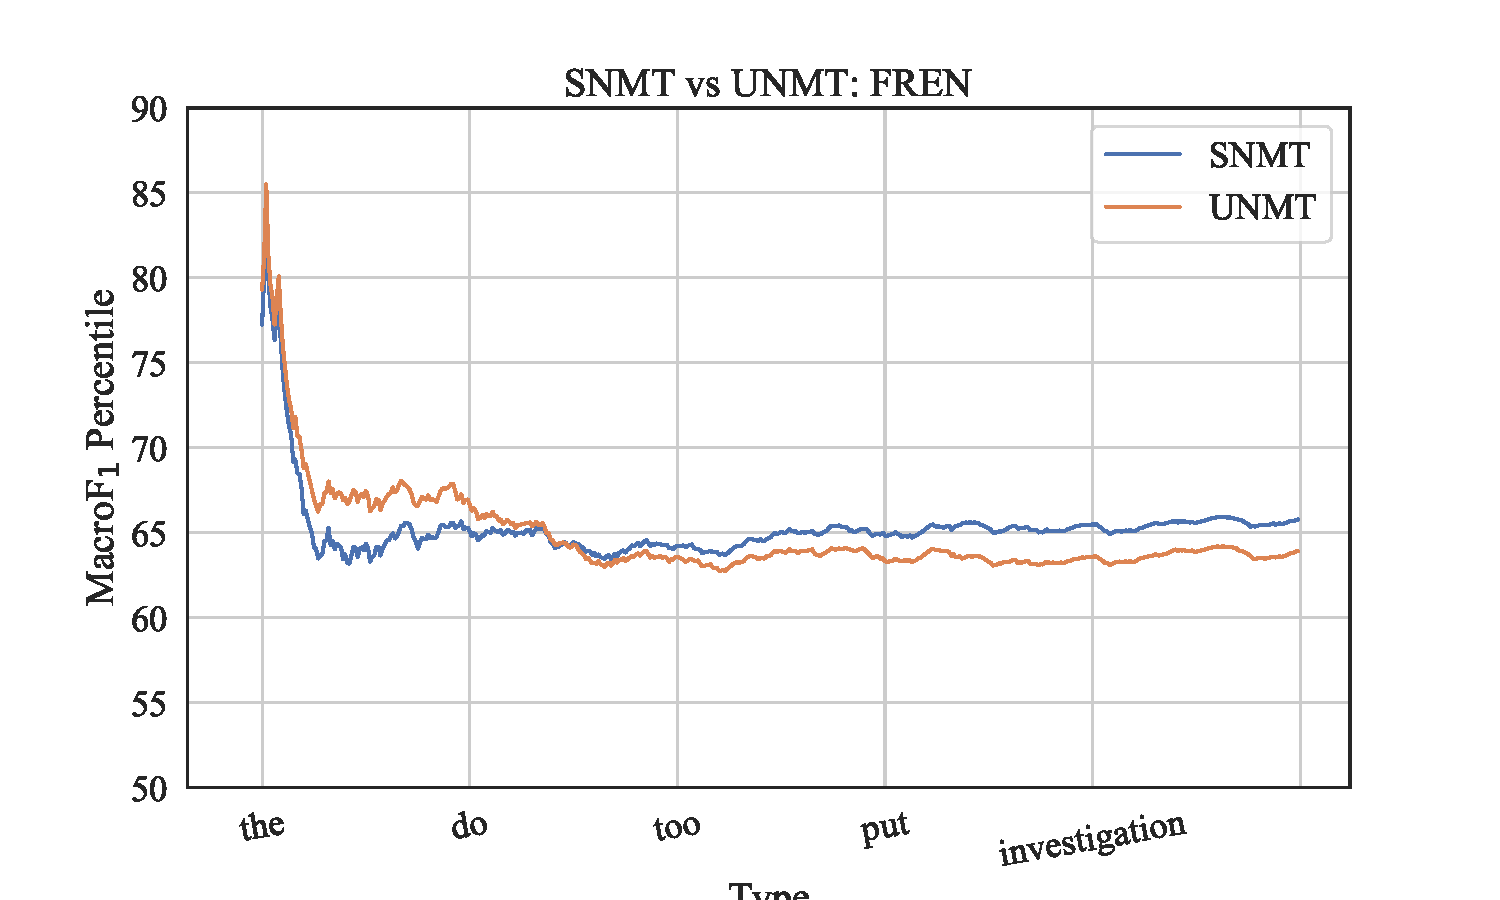
\includegraphics[width=\linewidth,trim={13mm 5mm 25mm 10mm},clip]{macroavg/s_unmt-fren-maf1.pdf}
    \end{subfigure}
    %\hfill 
    \begin{subfigure}[b]{0.49\linewidth}
    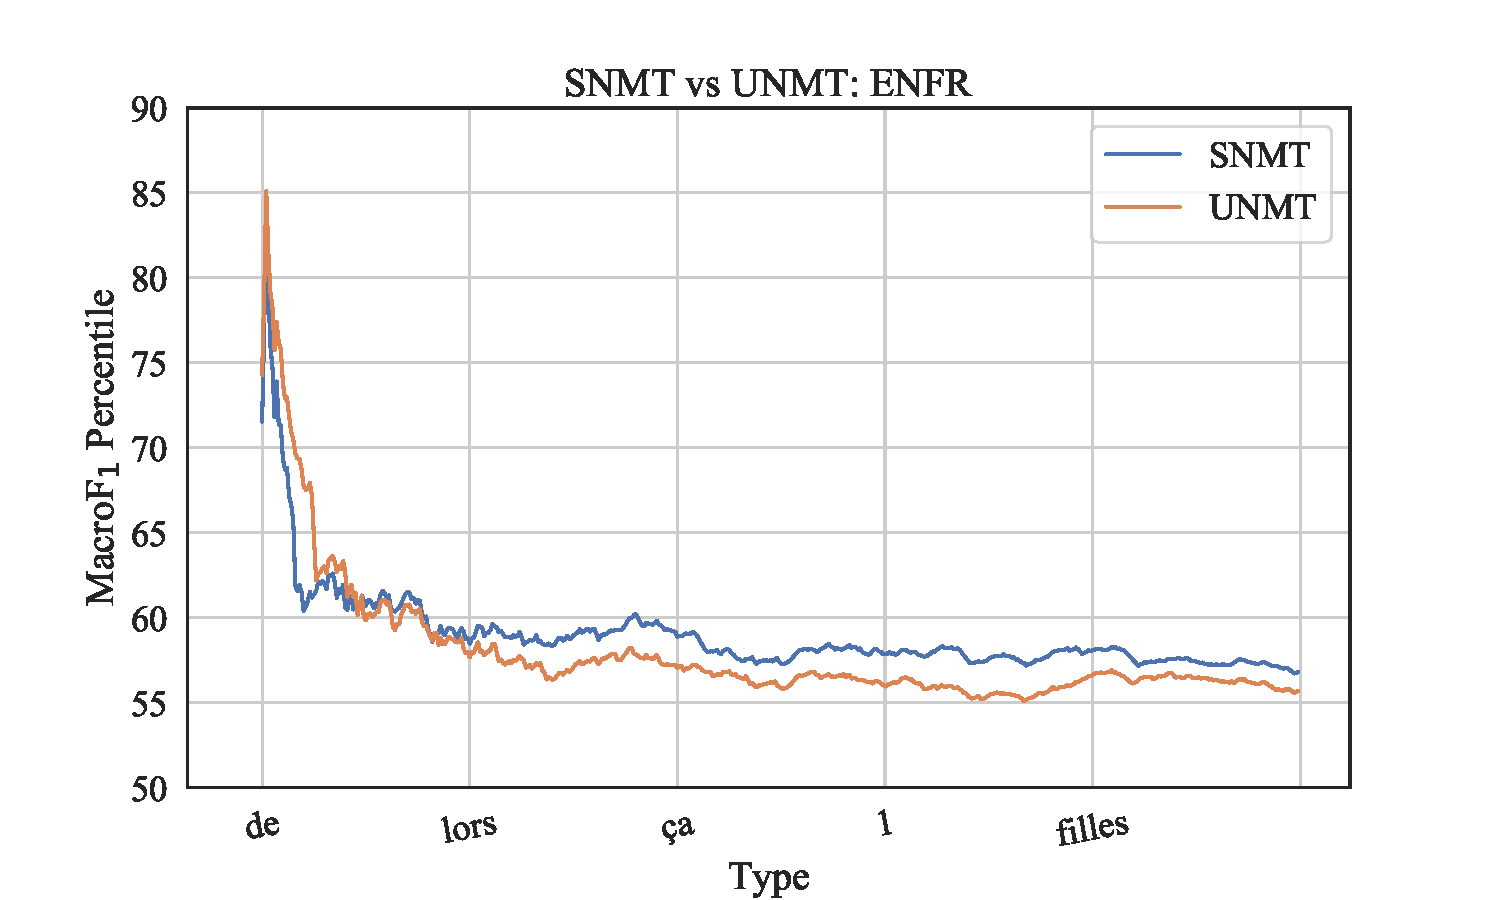
\includegraphics[width=\linewidth,trim={13mm 7mm 25mm 10mm},clip]{macroavg/s_unmt-enfr-maf1.pdf}
    \end{subfigure}
    
    \begin{subfigure}[b]{0.49\linewidth}
    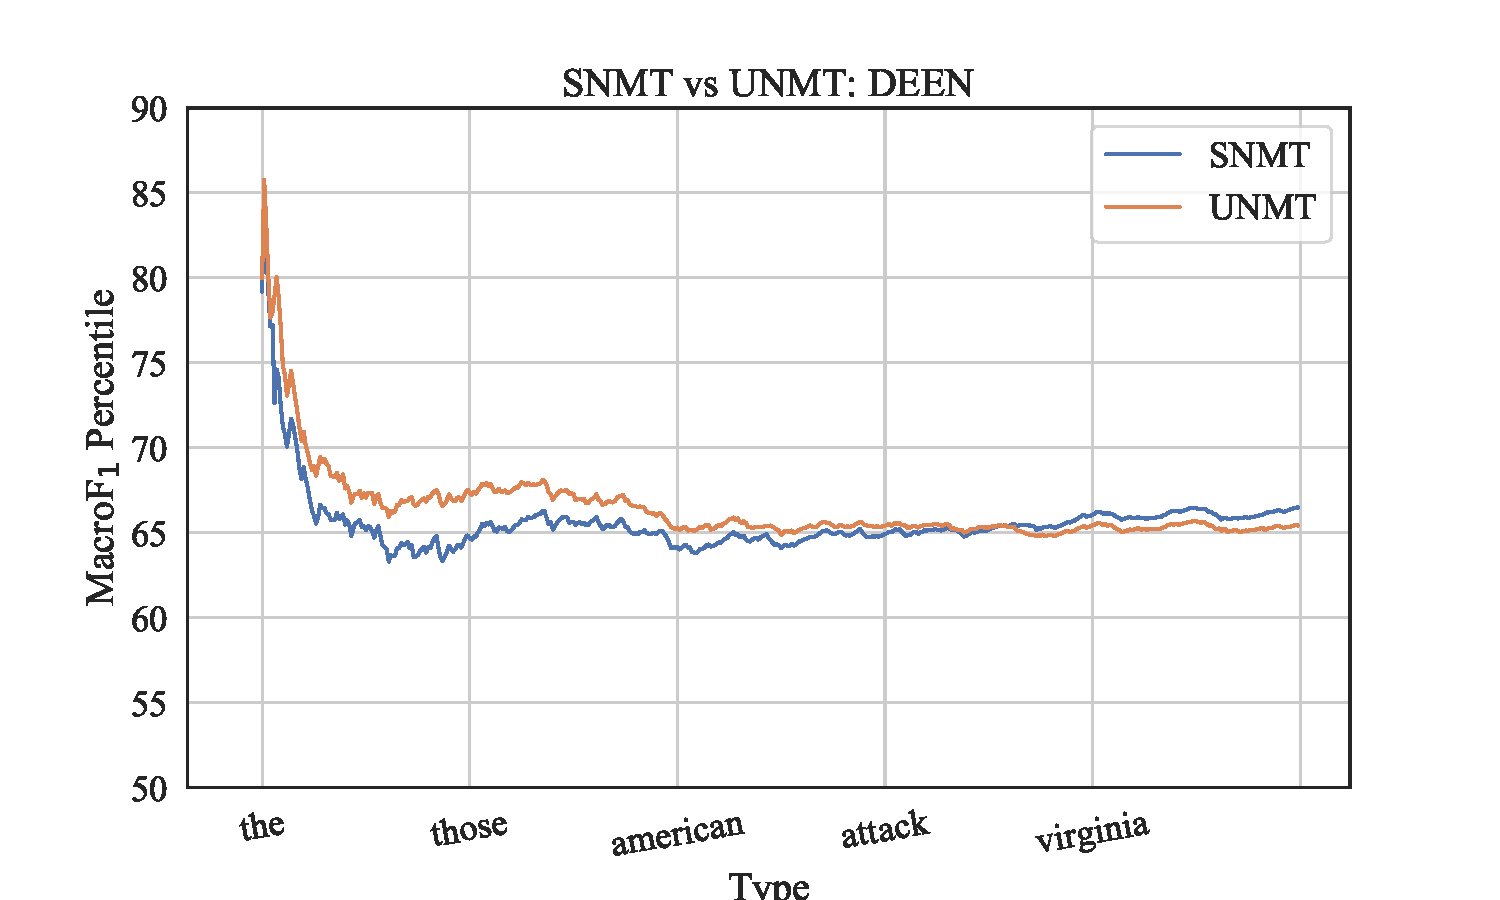
\includegraphics[width=\linewidth,trim={13mm 5mm 25mm 10mm},clip]{macroavg/s_unmt-deen-maf1.pdf}
    \end{subfigure}
    %\hfill 
    \begin{subfigure}[b]{0.49\linewidth}
    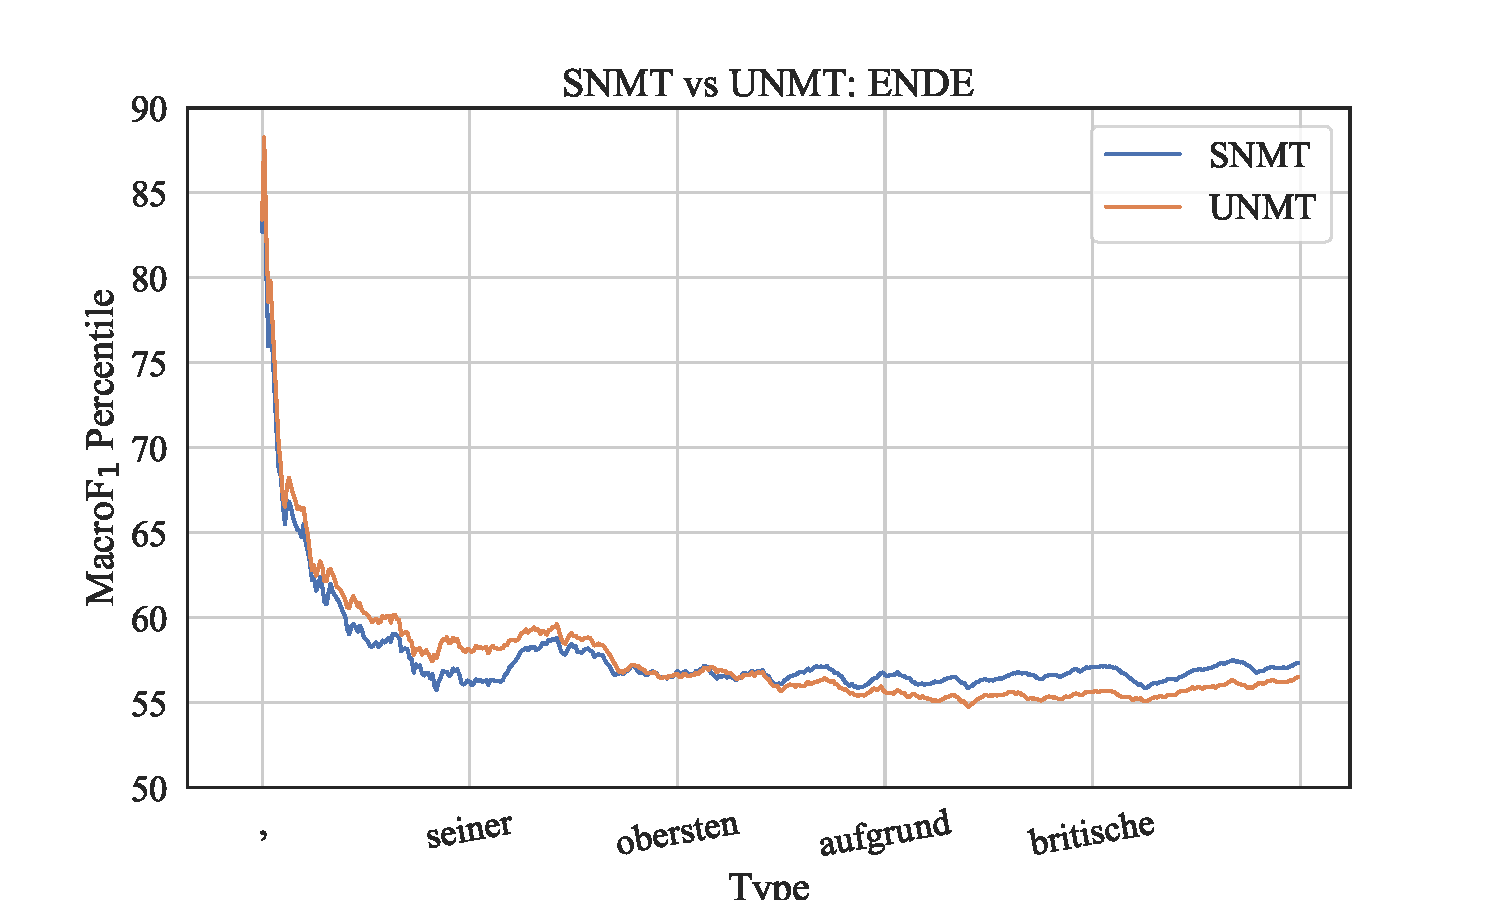
\includegraphics[width=\linewidth,trim={13mm 7mm 25mm 10mm},clip]{macroavg/s_unmt-ende-maf1.pdf}
    \end{subfigure}
    
    \begin{subfigure}[b]{0.49\linewidth}
    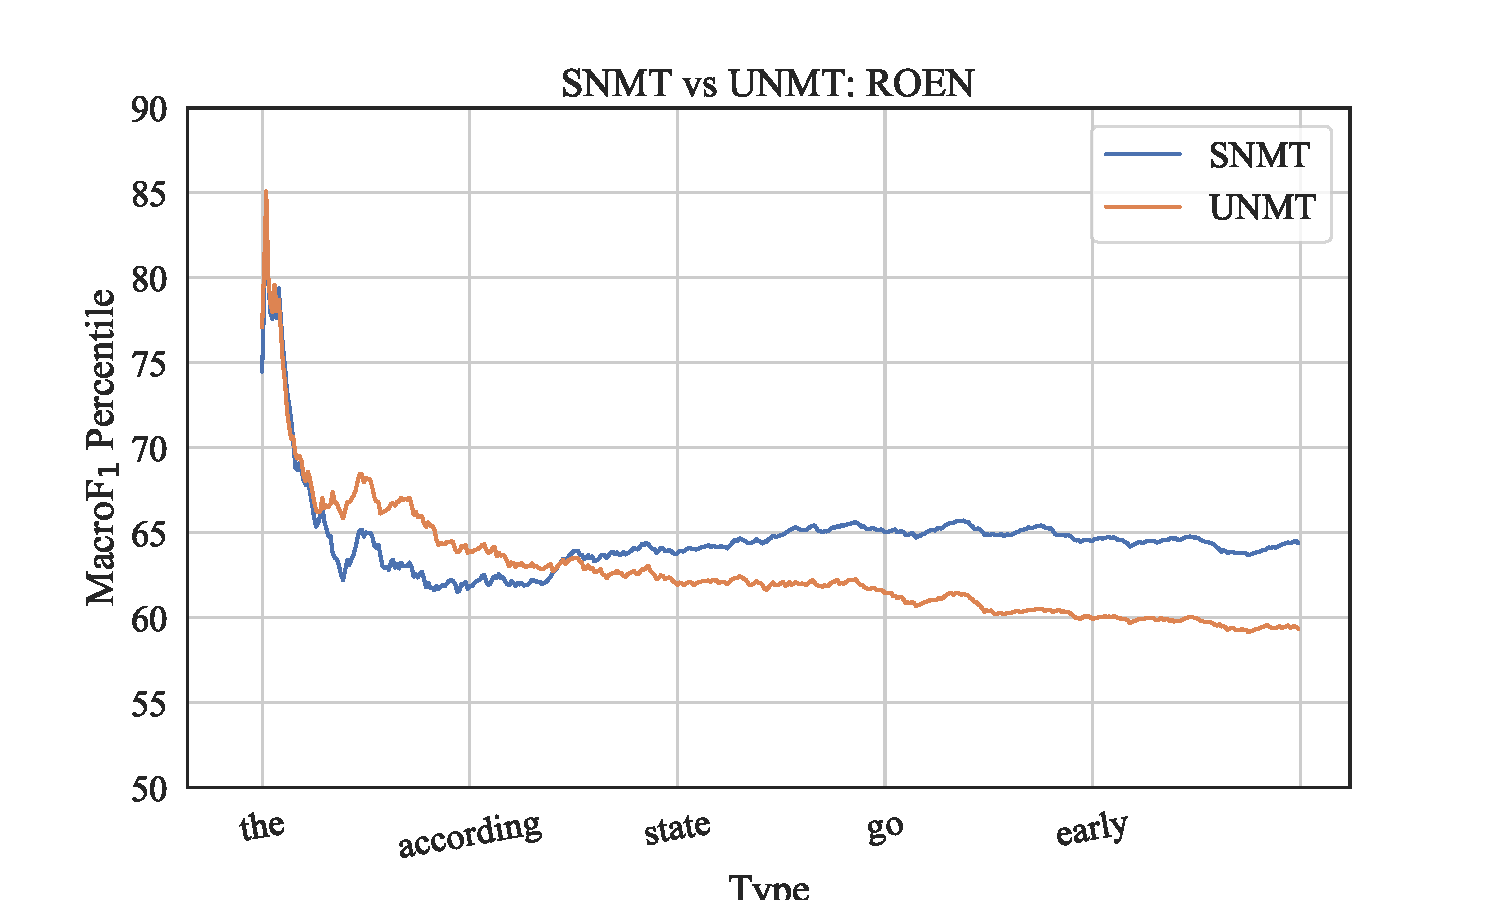
\includegraphics[width=\linewidth,trim={13mm 5mm 25mm 10mm},clip]{macroavg/s_unmt-roen-maf1.pdf}
    \end{subfigure}
    \begin{subfigure}[b]{0.49\linewidth}
      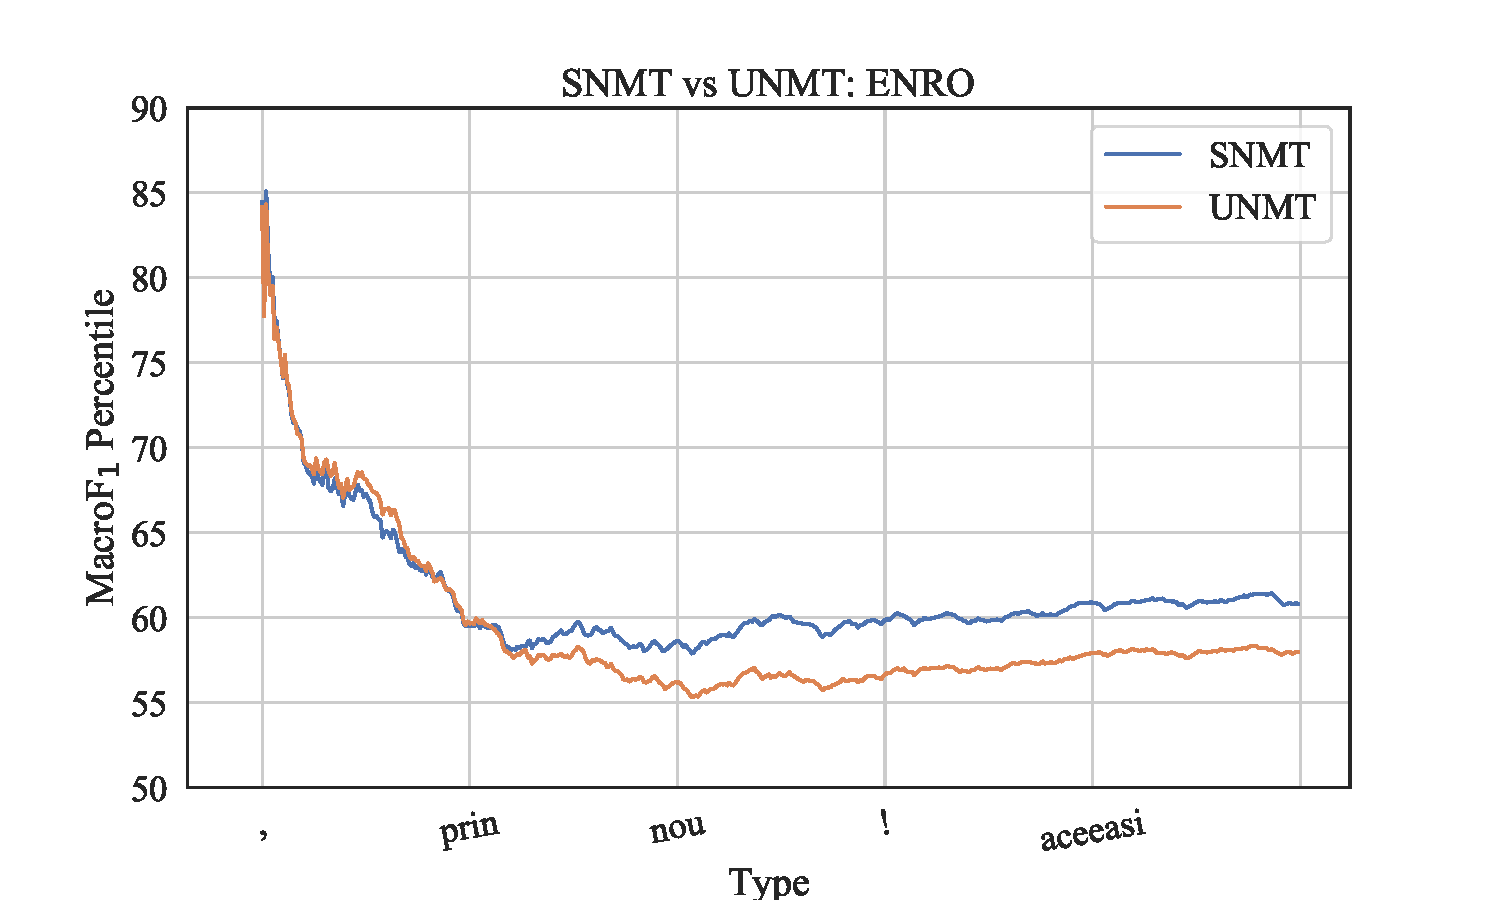
\includegraphics[width=\linewidth,trim={13mm 7mm 25mm 10mm},clip]{macroavg/s_unmt-enro-maf1.pdf}
      %\label{fig:snmt_vs_unmt_rest}
      %\caption{(Continued from Figure~\ref{fig:snmt_vs_unmt}) Visualization of \maf1 between SNMT and UNMT .  }
    \end{subfigure}
    
\caption{SNMT vs UNMT \maf1 on the most frequent 500 types.
UNMT outperforms SNMT on frequent types that are weighed heavily by \bleu\, however, SNMT is generally better than UNMT on rare types; hence, SNMT has a higher \maf1.
Only the most frequent 500 types are visualized in this figure.
}
\label{fig:snmt_vs_unmt}
\end{figure}



The UNMT models follow XLM's standard architecture and are trained with 5 million monolingual sentences for each language using a vocabulary size of 60,000. 
% using code base from \citet{rtg-xt20}
We train SNMT models for EN$\leftrightarrow$DE and select models with the most similar (or a slightly lower) BLEU as their UNMT counterparts on newstest2019. The DE-EN model selected is trained with 1 million sentences of parallel data and a vocabulary size of 64,000, and the EN-DE model selected is trained with 250,000 sentences of parallel data and a vocabulary size of 48,000. For EN$\leftrightarrow$FR and EN$\leftrightarrow$RO, we select SNMT models from submitted systems to WMT shared tasks that have similar or slightly lower BLEU scores to corresponding UNMT models, based on \textit{NewsTest2014} for EN$\leftrightarrow$FR and \textit{NewsTest2016} for EN$\leftrightarrow$RO. 

Figure~\ref{fig:snmt_vs_unmt}, which is a visualization of \maf1 for SNMT and UNMT models,  shows that UNMT is generally better than SNMT on frequent types, however, SNMT outperforms UNMT on the rest leading to a crossover point in \maf1 curves. 
Since \maf1 assigns relatively higher weights to infrequent types than in \bleu{}, SNMT gains higher \maf1 than UNMT while both have approximately the same \bleu{}, as reported in Table~\ref{tab:unmt_vs_snmt}.